\documentclass{article}
\usepackage[utf8x]{inputenc}
\usepackage[english,hebrew]{babel}
\usepackage{amsmath} 
\selectlanguage{hebrew}
\usepackage[top=2cm,bottom=2cm,left=2.5cm,right=2cm]{geometry}
\usepackage{graphicx} %package to manage images
\graphicspath{ {./images/} }
\usepackage{wrapfig}
\usepackage{empheq}

\title{נבחרת ישראל הצעירה בפיזיקה - מטלה 2 }
\author{איתי מור}
\begin{document}
\maketitle




\section*{מכניקה}
\subsection*{שאלה מהתרגול}
נתבונן בכוחות הפועלים על החוליות בכל צד:
    \begin{align*}
        \centering
        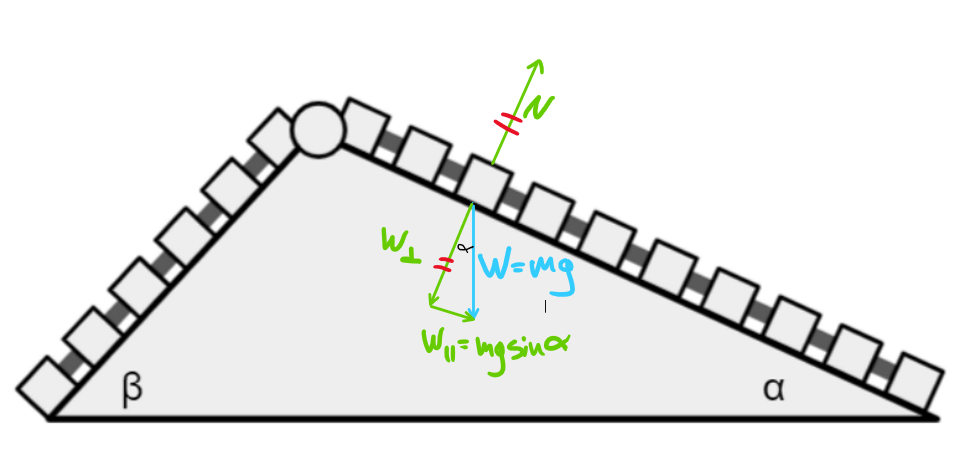
\includegraphics[scale=0.4]{images/from_tirgul_q5.png}
    \end{align*}
    
    \begin{align*}
        \centering
        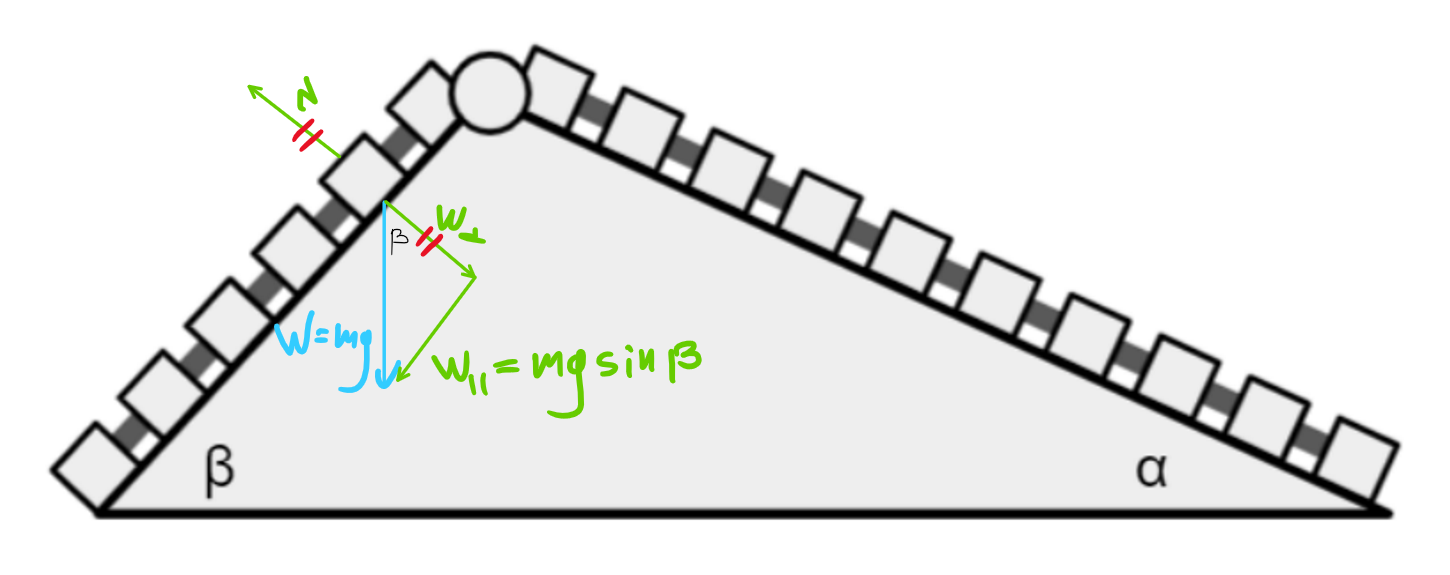
\includegraphics[scale=0.3]{images/from_tirgul_q5_b.png}
    \end{align*}
מכיוון שהכוחות המאונכים לטריז מבטלים אלו את אלו, הכוחות היחידים הפועלים על החוליות בשרשרת הם הכוחות הפועלים במקביל לטריז.\\
נסמן את אורך הצלע השמאלית של הטריז ב
$a$
ואת הצלע הימנית של הטריז ב
$b$.\\
ע"פ משפט הסינוסים:
\begin{equation*}
    \frac{a}{\sin \alpha} = \frac{b}{\sin \beta}
\end{equation*}
נכפיל את שני האגפים ב
$n$
ונקבל את כמות החוליות שיש בכל צד לחלק לסינוס הזווית שליד אותה הפאה של הטריז:
\begin{equation*}
    \frac{an}{\sin \alpha} = \frac{bn}{\sin \beta}
\end{equation*}
נסמן:
\begin{equation*}
    an\sin{\beta} = bn \sin{\alpha} = k
\end{equation*}
\\
נחשב את סכום הכוחות הפועלים על השרשרת )לצד שמאל(:
\begin{equation*}
    \Sigma{\vec{F}} = an \cdot mg\sin{\beta} - bn \cdot mg\sin{\alpha} = k(mg - mg) = 0
\end{equation*}
ולכן גם התאוצה היא $0$, כלומר השרשרת נעה במהירות קבועה )או במנוחה(.




\newpage
\subsection*{זינוק בירידה - המשך}

\newpage
\subsection*{הרמת משקולות}
\begin{align*}
    \centering
    \fbox{
        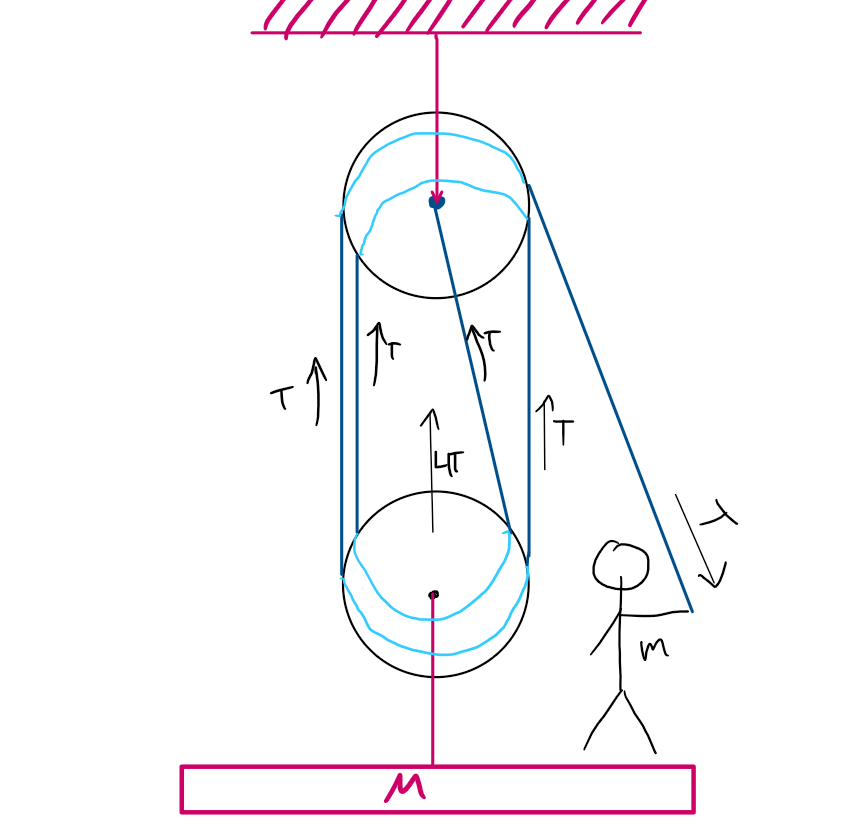
\includegraphics[scale=0.4]{images/t2_q2_diagram.png}
    }
\end{align*}
מהשרטוט ניתן לראות ש-
\begin{flalign*}
    &4T = (m+M)g&&
    \\&T = (m+M)\frac{g}{4}&&
\end{flalign*}






\newpage
\section*{חשבון דיפרנציאלי}
\subsection*{כללי נגזרות}
\begin{enumerate}
    \item כלל המכפלה: \\
    נפרק את מכפלת הפונקציות כמתואר באיור הבא: 
    \begin{align*}
        \centering
        \fbox{
            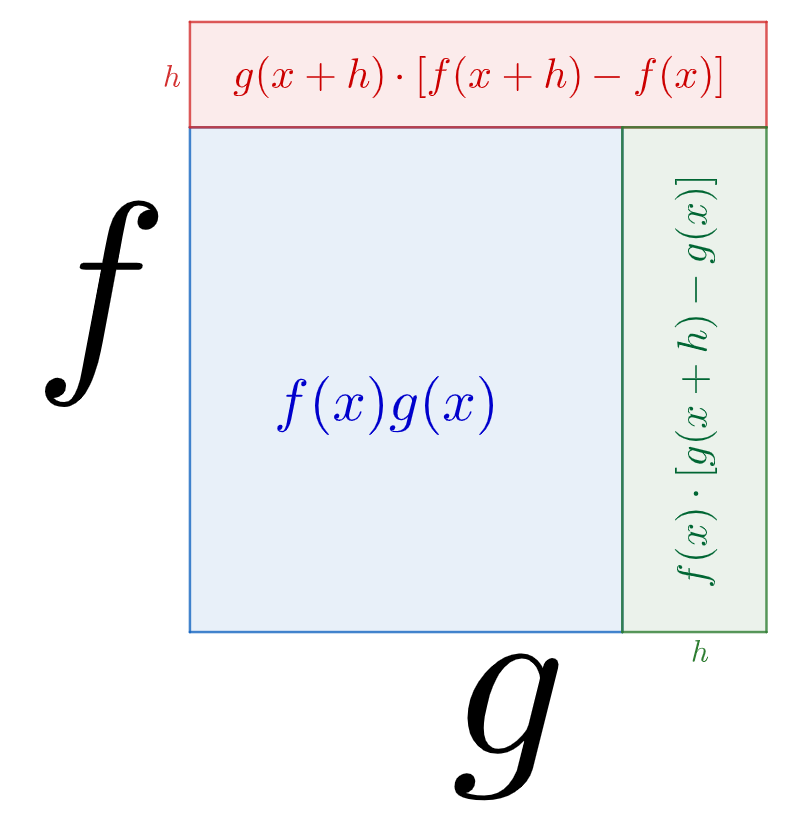
\includegraphics[scale=0.4]{images/derivative_drawing.png}
        }
    \end{align*}
    
    \begin{flalign*}
      \frac{d (f g)}{d x} = \lim_{h \to 0}{\frac{f(x+h)g(x+h) - f(x)g(x)}{h}} 
      = \lim_{h \to 0}{ \frac{ g(x+h) \cdot \left[ f(x+h)-f(x) \right] + f(x) \cdot \left[ g(x+h) - g(x) \right]}{h} } &&
    \end{flalign*}
    \begin{flalign*}
        = \frac{d f}{d x} \cdot \lim_{h \to 0}{g(x+h)}  + \frac{d g}{d x} \cdot \lim_{h \to 0}{f(x)} 
        = \frac{d f}{d x} g + \frac{d g}{d x} f&&
    \end{flalign*}

    \item כלל המנה:
    \begin{flalign*}
        \frac{d \left( \frac{f}{g}\right)}{d x} = \lim_{h \to 0}{\frac{\frac{f(x+h)}{g(x+h)} - \frac{f(x)}{g(x)}}{h}}
        = \lim_{h \to 0}{\frac{\frac{f(x+h)g(x) - f(x)g(x+h)}{g(x)g(x+h)}}{h}}
        = \frac{\displaystyle \lim_{h \to 0}{\frac{f(x+h)g(x)-g(x+h)f(x)}{h}}}{\displaystyle \lim_{h \to 0}{g(x)g(x+h)}}&&
    \end{flalign*}
    \begin{flalign*}
        = \frac{\displaystyle \lim_{h \to 0}{\frac{f(x+h)g(x) - g(x+h)f(x) + g(x)f(x) - g(x)f(x)}{h}}}{g^2(x)}&&
    \end{flalign*}
    \begin{flalign*}
        = \frac{\displaystyle \lim_{h \to 0}{g(x) \cdot [f(x+h) - f(x)]} - \lim_{h \to 0}{f(x) \cdot [g(x+h) - g(x)]}}{g^2(x)}
        = \frac{f(x) \frac{d f}{d x} - g(x) \frac{d g}{d x}}{g^2(x)}&&
    \end{flalign*}
\end{enumerate}




\subsection*{מן הפח אל הפחית}
\begin{enumerate}
  \item הכוונה בעובי קטן מאוד היא עובי קטן מאוד ביחס לרדיוס הפחית ולגובה הפחית כדי שהעובי לא ישפיע על נפח הפחית:
  \begin{align*}
      width \ll r \\
      width \ll h
  \end{align*}
    



  \item קל לראות שעלות הייצור של פחית תלוייה ישירות בשטח הפנים שלה )מכיוון ששטח הפנים כפול עובי הפחית כפול עלות פח נותן את עלות הייצור( .\\
  נפח הפחית הוא $V = \pi h r^2$,
  כלומר:

  \begin{equation*}
      h = \frac{V}{\pi r^2}
  \end{equation*}

  שטח הפנים של הפחית כתלות ברדיוס הוא: 
  \begin{equation*}
      A(r) =  2\pi r\left( h+r \right) = 2\pi hr + 2\pi r^2
  \end{equation*}
  נציב את הערך של הגובה שקיבלנו:
    \begin{equation*}
      A(r) =  2\pi r \cdot \frac{V}{\pi r^2} + 2\pi r^2 = \frac{2V}{r} +2\pi r^2
    \end{equation*}
  נגזור את הפונקציה ונשווה ל-0 כדי לקבל את שטח הפנים המינימאלי שיוצר נפח $V$:

  \begin{equation*}
    A'(h) = -\frac{2V}{r^2} + 4\pi r = 0
  \end{equation*}
  \begin{equation*}
      r^3 = \frac{V}{2\pi}
  \end{equation*}
  \begin{equation*}
      r = \sqrt[\leftroot{-2}\uproot{2}3]{\frac{V}{2\pi}}
  \end{equation*}
    \begin{equation*}
      V = h\pi r^2
  \end{equation*}
  \begin{equation*}
      V = h\pi\sqrt[\leftroot{-2}\uproot{2}3]{\frac{V^2}{4\pi^2}} = h\sqrt[\leftroot{-2}\uproot{2}3]{\frac{V^2\pi}{4}}
  \end{equation*}
    \begin{equation*}
        h = \frac{V}{\sqrt[\leftroot{-2}\uproot{2}3]{\frac{V^2\pi}{4}}}
        = \sqrt[\leftroot{-2}\uproot{2}3]{\frac{V^3}{\frac{V^2\pi}{4}}}
        = \sqrt[\leftroot{-2}\uproot{2}3]{\frac{4V}{\pi}}
    \end{equation*}

    \begin{equation*}
        \frac{r}{h} =\sqrt[\leftroot{-2}\uproot{2}3]{\frac{\frac{V}{2\pi}}{\frac{4V}{\pi}}} = \sqrt[\leftroot{-2}\uproot{2}3]{\frac{1}{8}} = \frac{1}{2}
    \end{equation*}
    כלומר היחס בין הרדיוס לגובה שנותן את העלות המינימלית הוא $1 : 2$

    \item בפחית קוקה קולה רגילה,היחס בין הרדיוס לגובה הוא $\frac{6}{31}$:
    \begin{align*}
        \centering
        \fbox{
            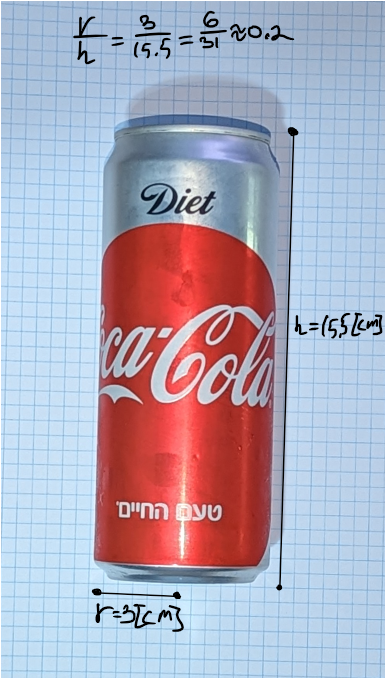
\includegraphics[scale=0.4]{images/can_measures.png}
        }
    \end{align*}
    נסמן את פונקצית עלות הייצור של הפחית כתלות ברדיוס ב
    $f(r)$,
    את עובי הבסיסים ב
    $w_b$
    ואת עובי המעטפת ב
    $w_s$.
    \begin{flalign*}
        f(r)=2\pi r^2 w_b + 2\pi r h w_s&&
    \end{flalign*}
    מנוסחאת נפח של פחית נקבל-
    \begin{flalign*}
        &V = \pi r^2 h&&
        \\&h = \frac{V}{\pi r^2}&&
    \end{flalign*}
    נציב בפונקציית עלות הייצור ונקבל:
    \begin{flalign*}
        &f(r) = 2\pi r^2 w_b + \frac{2\pi r V w_s}{\pi r^2} = 2\pi r^2 w_b +\frac{2V}{r}w_S&&
    \end{flalign*}
    נגזור את הפונקציה ונשווה ל-0 כדי למצוא נקודת קיצון:
    \begin{flalign*}
        &\frac{d\,f}{d\,r} = 4\pi r w_b - \frac{2V}{r^2} w_s = 0&&
      \\&4\pi r w_b = \frac{2V}{r^2}w_s&&
      \\&\frac{2\pi r^3}{V} = \frac{w_s}{w_b}&&
      \\&\frac{2\pi r^3}{\pi r^2 h} = \frac{w_s}{w_b}&&
      \\&\frac{2r}{h} = \frac{w_s}{w_b}&
      \\&\frac{w_s}{w_b} = \frac{12}{31} \approx \frac{2}{5}
    \end{flalign*}
    זוהי בהכרח נק' מינימום מכיוון שגם כשהיחס בין הרדיוס לגובה שואף לאינסוף )הרדיוס שואף לאינסוף והגובה שואף לאפס( עלות הייצור שואפת לאינסוף וגם כשהיחס בין הרדיוס לגובה שואף לאפס )הגובה שואף לאינסוף והרדיוס שואף לאפס( עלות הייצור שואפת לאינסוף:
    \begin{flalign*}
        \lim_{r \to \infty}{2\pi r(\frac{V}{2\pi r}+r)} = \infty&&
    \end{flalign*}
    \begin{flalign*}
        \lim_{r \to 0^+}{2\pi r(\frac{V}{\pi r^2}+r)} = 2\pi\lim_{r \to 0}{r^2 + \frac{V}{\pi r}} = 2\pi(0 +\infty) = \infty&&
    \end{flalign*}
\end{enumerate}





\newpage
\subsection*{באש...}
אם נשקף את האש ביחס לים, נוכל למתוח קטע בין שגיא לשיקוף, וזה יהיה המרחק הקצר ביותר בין השיקוף לשגיא.\\
מכיוון שקו המים הוא אנך אמצעי לקטע שבין האש לשיקוף, המרחקים מנק' החיתוך של הקטע שמתחנו מקודם, לאש ולשיקוף של האש, שווים:
\begin{align*}
    \centering
    \fbox{
        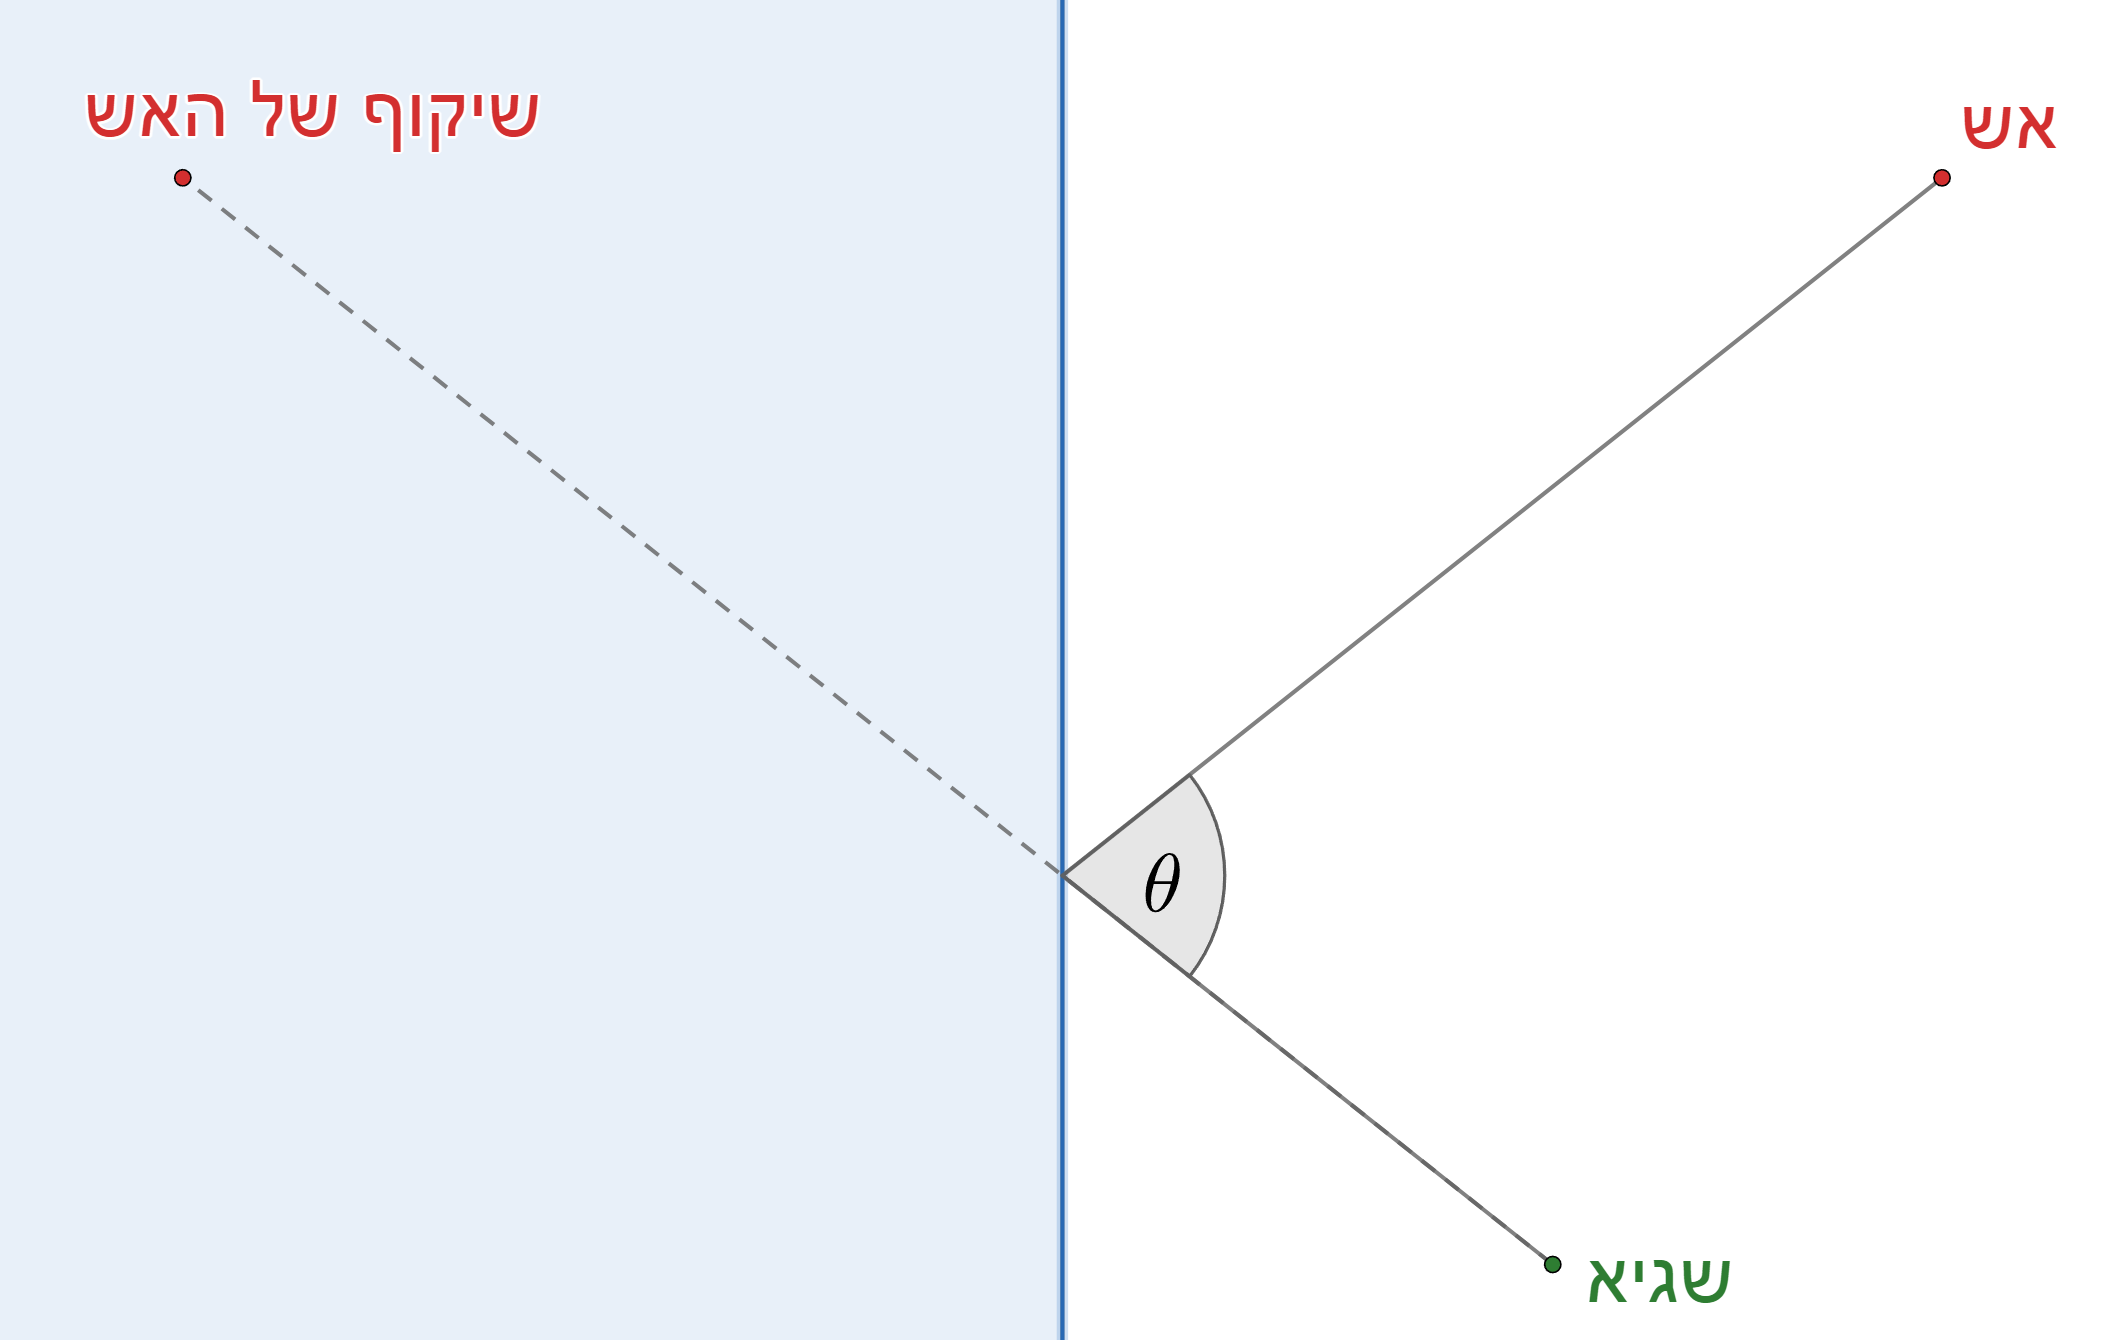
\includegraphics[scale=0.4]{images/geogebra-export.png}
    }
\end{align*}
לכן אותה נק' חיתוך היא בהכרך הנקודה שממנה שגיא לוקח מים.
\begin{align*}
    \centering
    \fbox{
        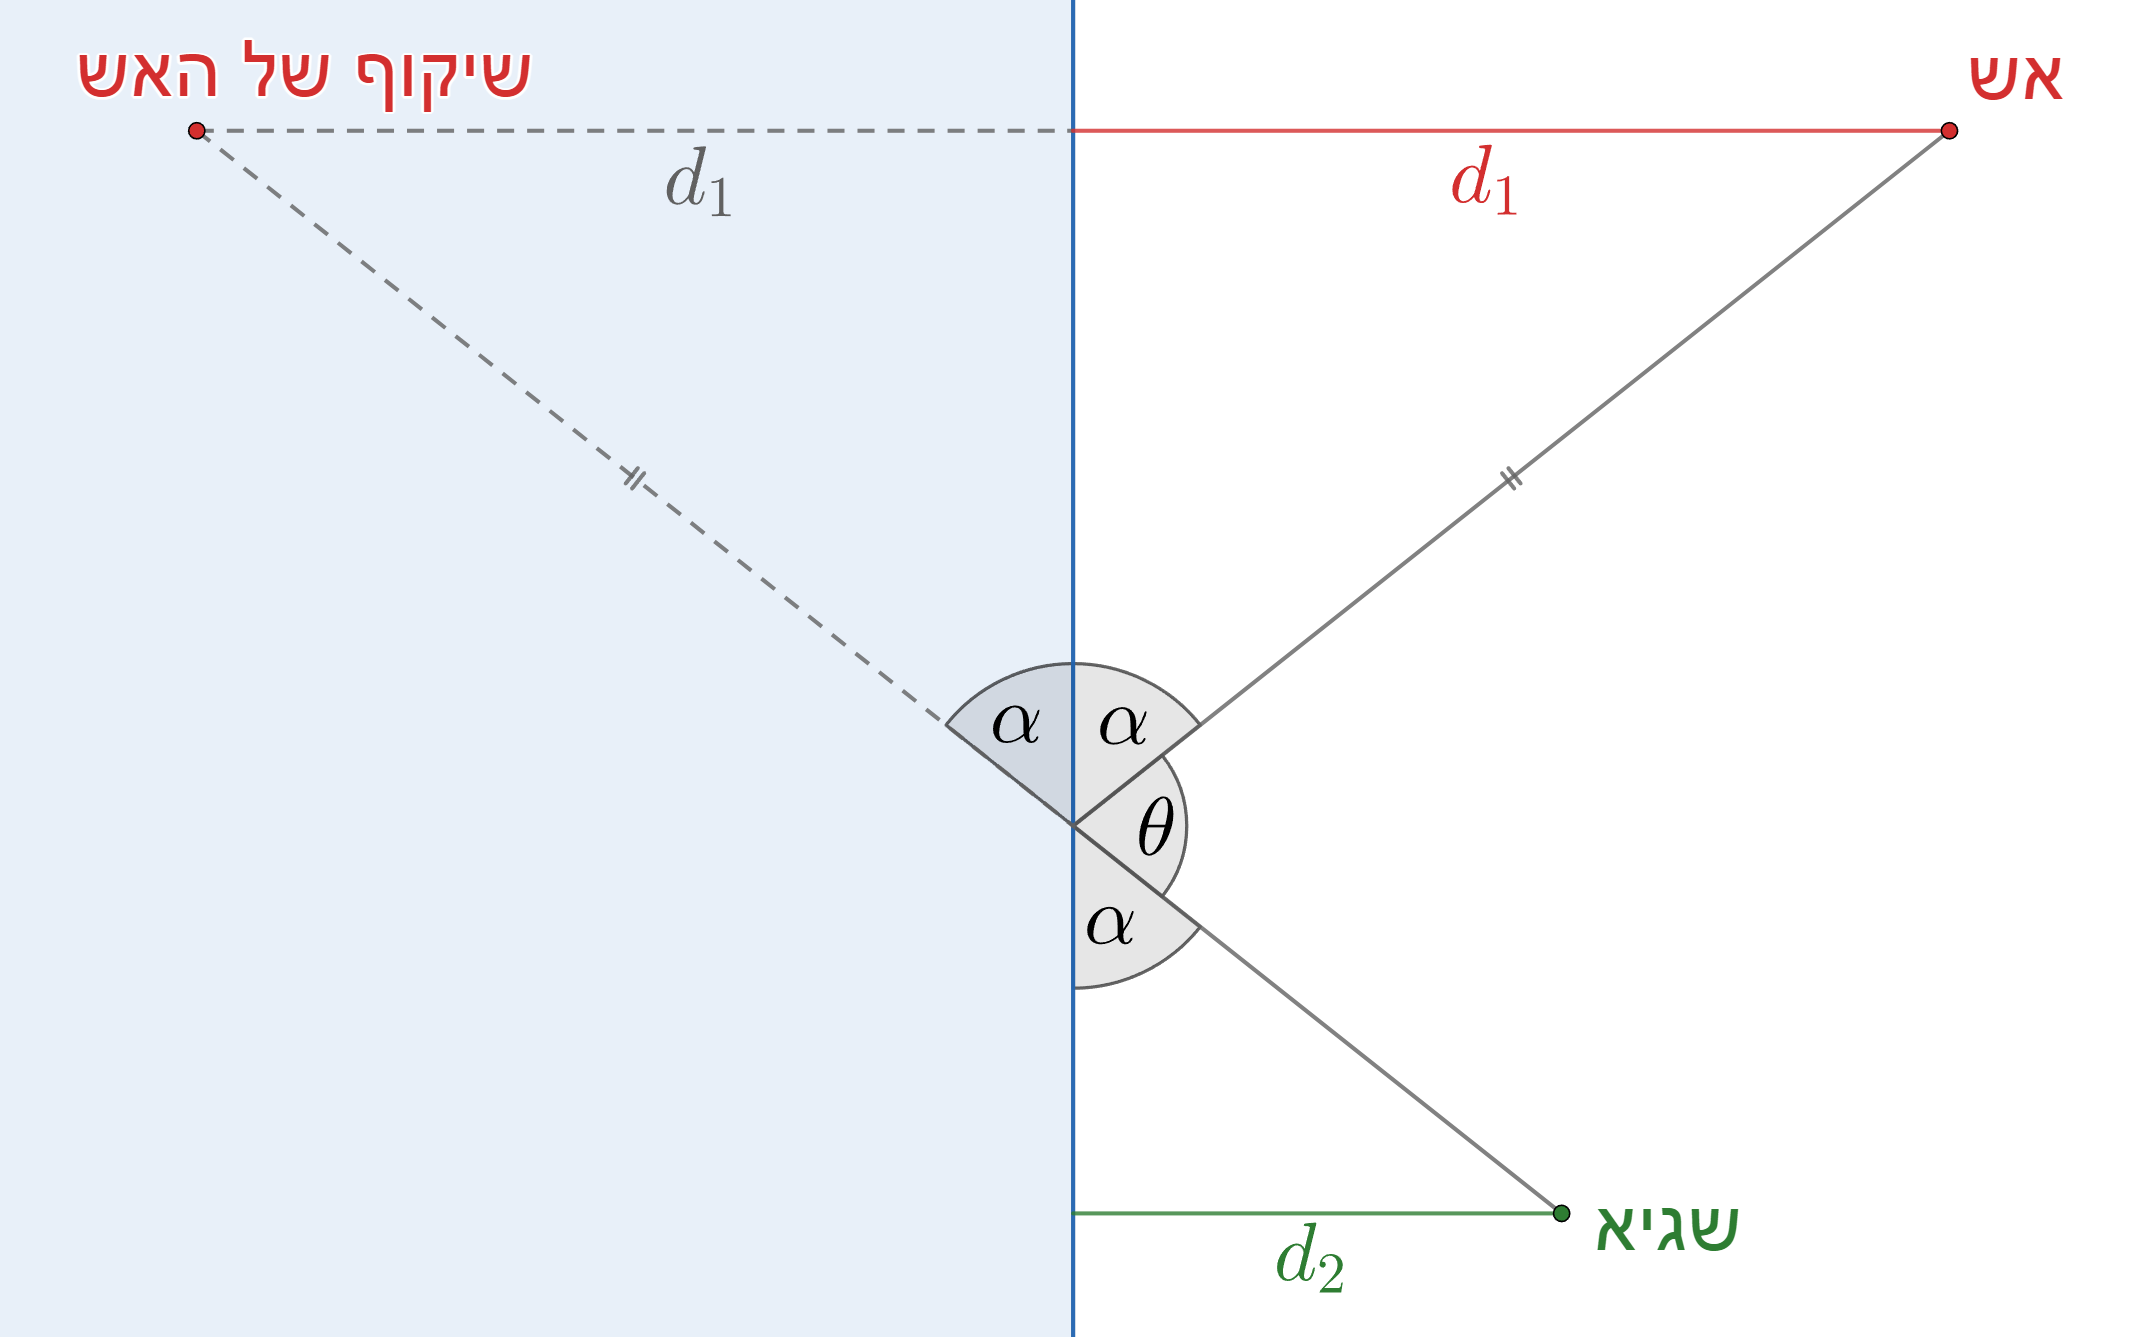
\includegraphics[scale=0.4]{images/on_fire_figure_with_angles.png}
    }
\end{align*}
זווית $\alpha$ שווה ל-$\frac{\pi - \theta}{2}$.\\
נסמן את המרחק על ציר ה
$y$ 
בין נק' לקיחת המים לאש ב
$y_1$,
ואת המרחק על ציר ה
$y$
בין נק' לקיחת המים לשגיא ב
$y_2$.\\
בנוסף נסמן את המרחק הכולל ב
$y_1+y_2 = h$
\begin{equation*}
    \tan (\alpha) = \frac{y_1}{d_1}
\end{equation*}
\begin{equation*}
    \tan (\alpha) = \frac{y_2}{d_2}
\end{equation*}
\\
\\
\begin{equation*}
    y_1 + y_2 = (d_1 + d_2)\tan (\alpha) 
\end{equation*}
\begin{equation*}
    \frac{h}{d_1 + d_2} = \tan (\alpha) 
\end{equation*}
\begin{equation*}
    \alpha = \tan ^ {-1} \left( \frac{h}{d_1 + d_2} \right)
\end{equation*}
\begin{equation*}
    \frac{\pi}{2} - \frac{\theta}{2} = \tan ^ {-1}\left( \frac{h}{d_1 + d_2} \right)
\end{equation*}
\begin{equation*}
    \theta = \pi - 2\tan ^ {-1} \left( \frac{h}{d_1 + d_2} \right)
\end{equation*}


\newpage
\subsection*{ובמים...}
נניח שקיים מסלול A בין שגיא לילד הטובע.
כעת נסתכל על מסלול B, שחותך את קו החוף במרחק 
$dy$
ששואף לאפס ממסלול A.\\
מכיוון שהמרחק על קו החוף בין המסלולים שואף לאפס, גם הזוויות בין המסלולים ישאפו לאפס:
\begin{align*}
    \centering
    \fbox{
        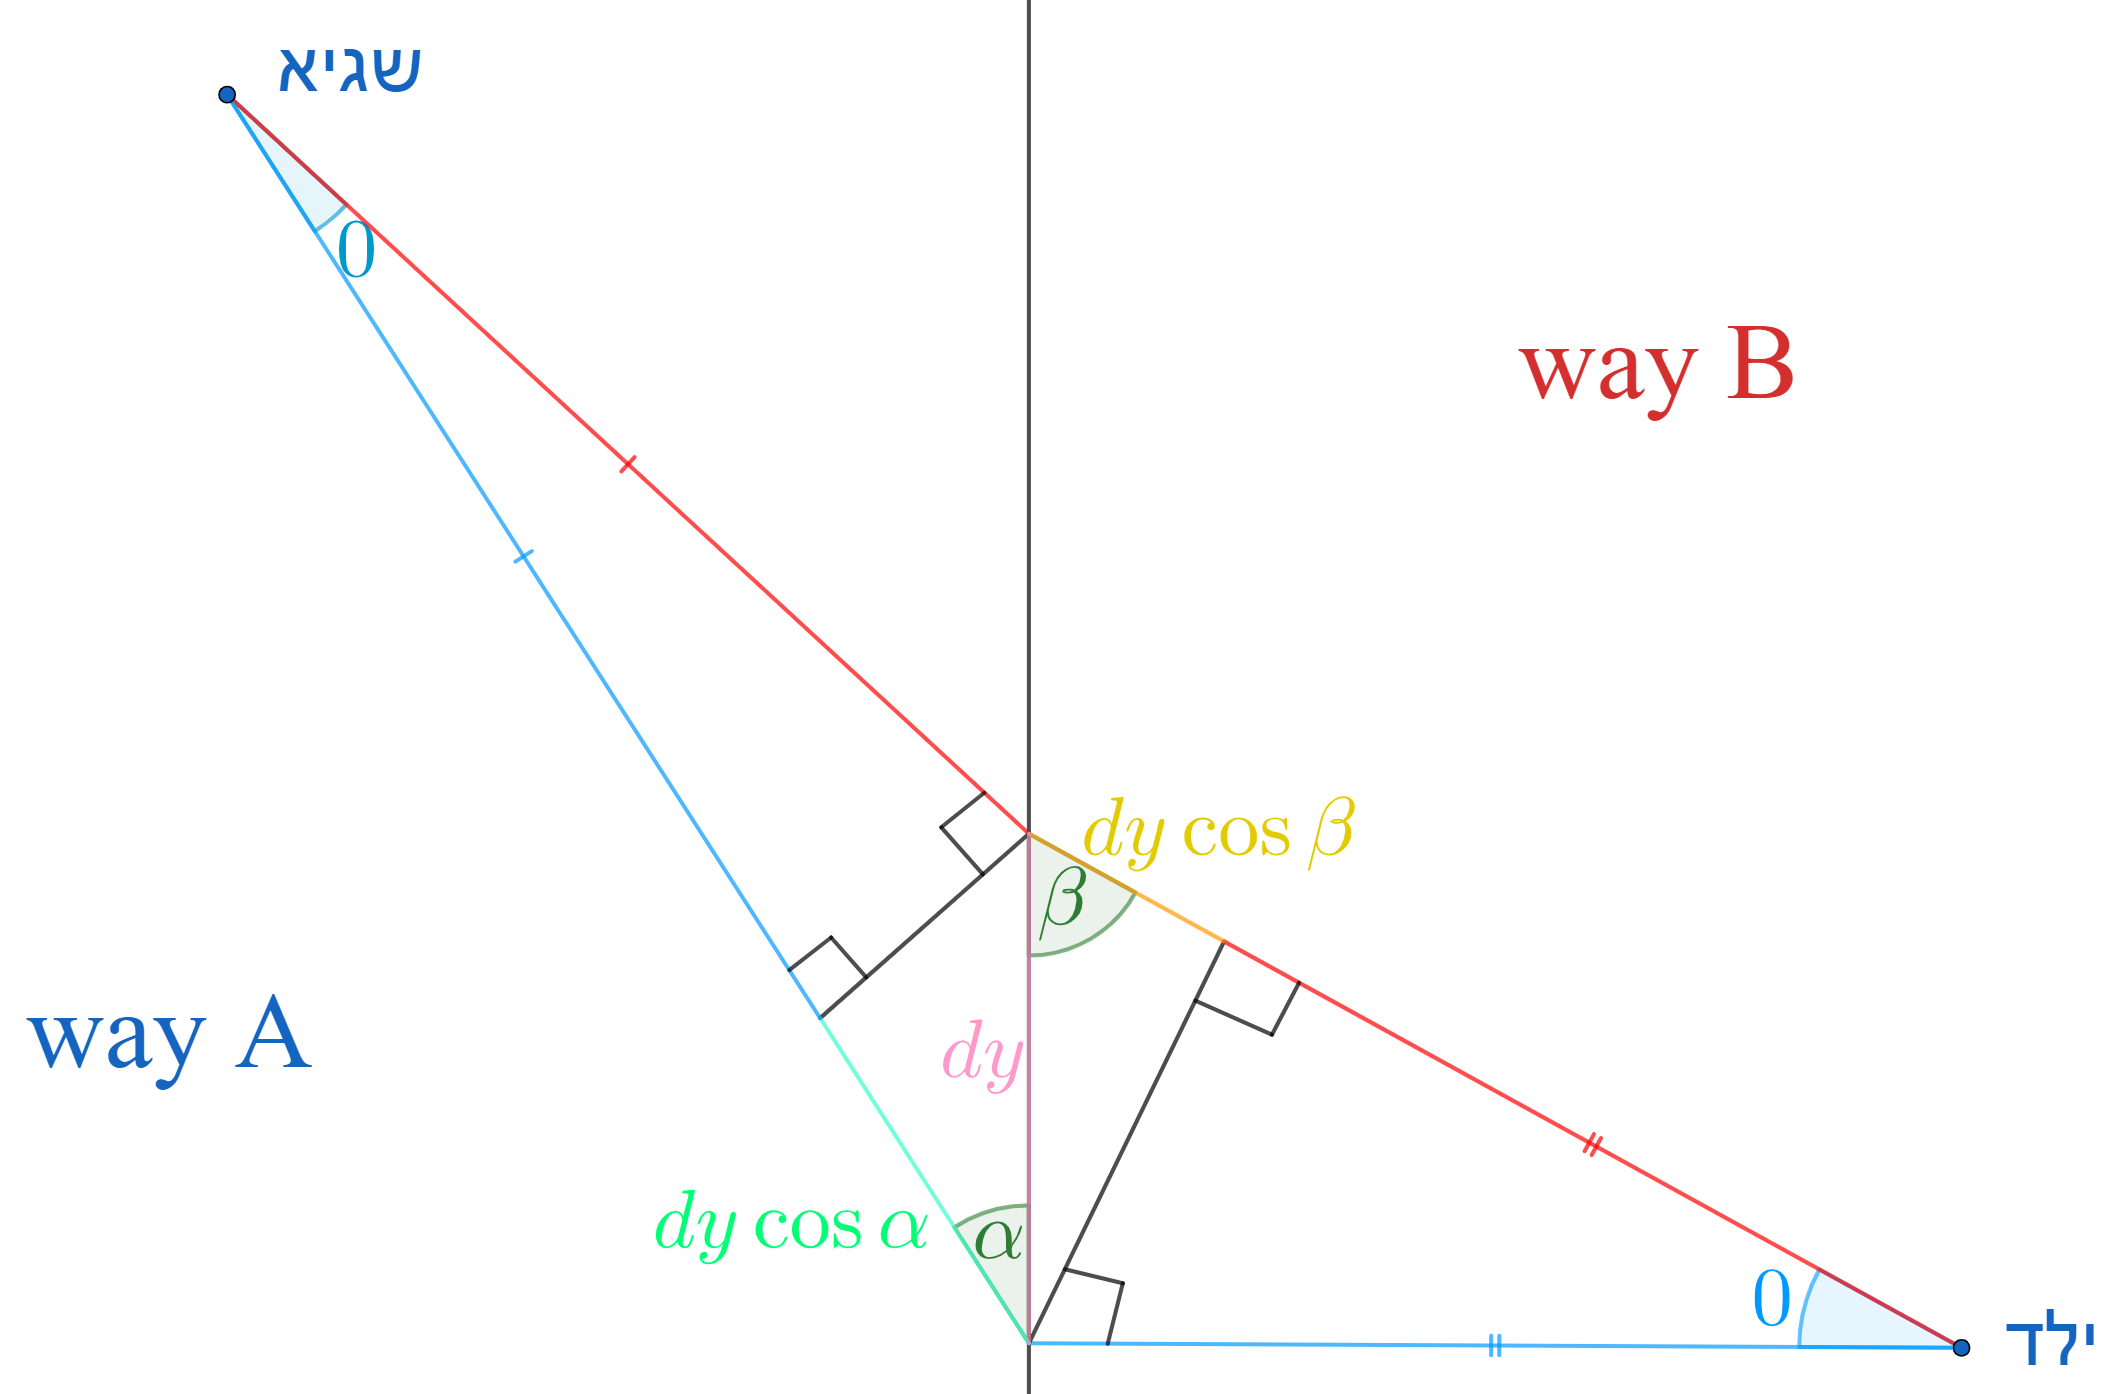
\includegraphics[scale=0.8]{images/and_in_the_water_diagram.png}
    }
\end{align*}
לכן הקטע הצהוב זה הקטע שמתווסף למסלול, והקטע הטורקיז זה הקטע שיורד מהמסלול.\\
נרצה לחשב את השינוי בזמן שלוקח לשגיא להגיע לילד ביחס לשינוי ב
$dy$.
הזמן שמתווסף הוא 
$u\cdot dy\cos \beta$,
והזמן שיורד הוא
$v\cdot dy\cos \alpha$.\\
לכן:
\begin{flalign*}
    &dT=dy(u\cos{\beta} - v\cos{\alpha})&&\\
    &\frac{dT}{dy} = u\cos{\beta} - v\cos{\alpha}&&
\end{flalign*}
אנחנו מחפשים את נקודת המינימום, כלומר נקודה שבה כש $dy$ שואף לאפס
גם $dT$ שואף לאפס.
\begin{flalign*}
    &\frac{dT}{dy} = u\cos{\beta} - v\cos{\alpha} = 0&&\\
    &u\cos{\beta} = v\cos{\alpha}&&
\end{flalign*}

בנוסף, קיים עוד קשר בין שתי הזוויות:
\begin{align*}
    \centering
    \fbox{
        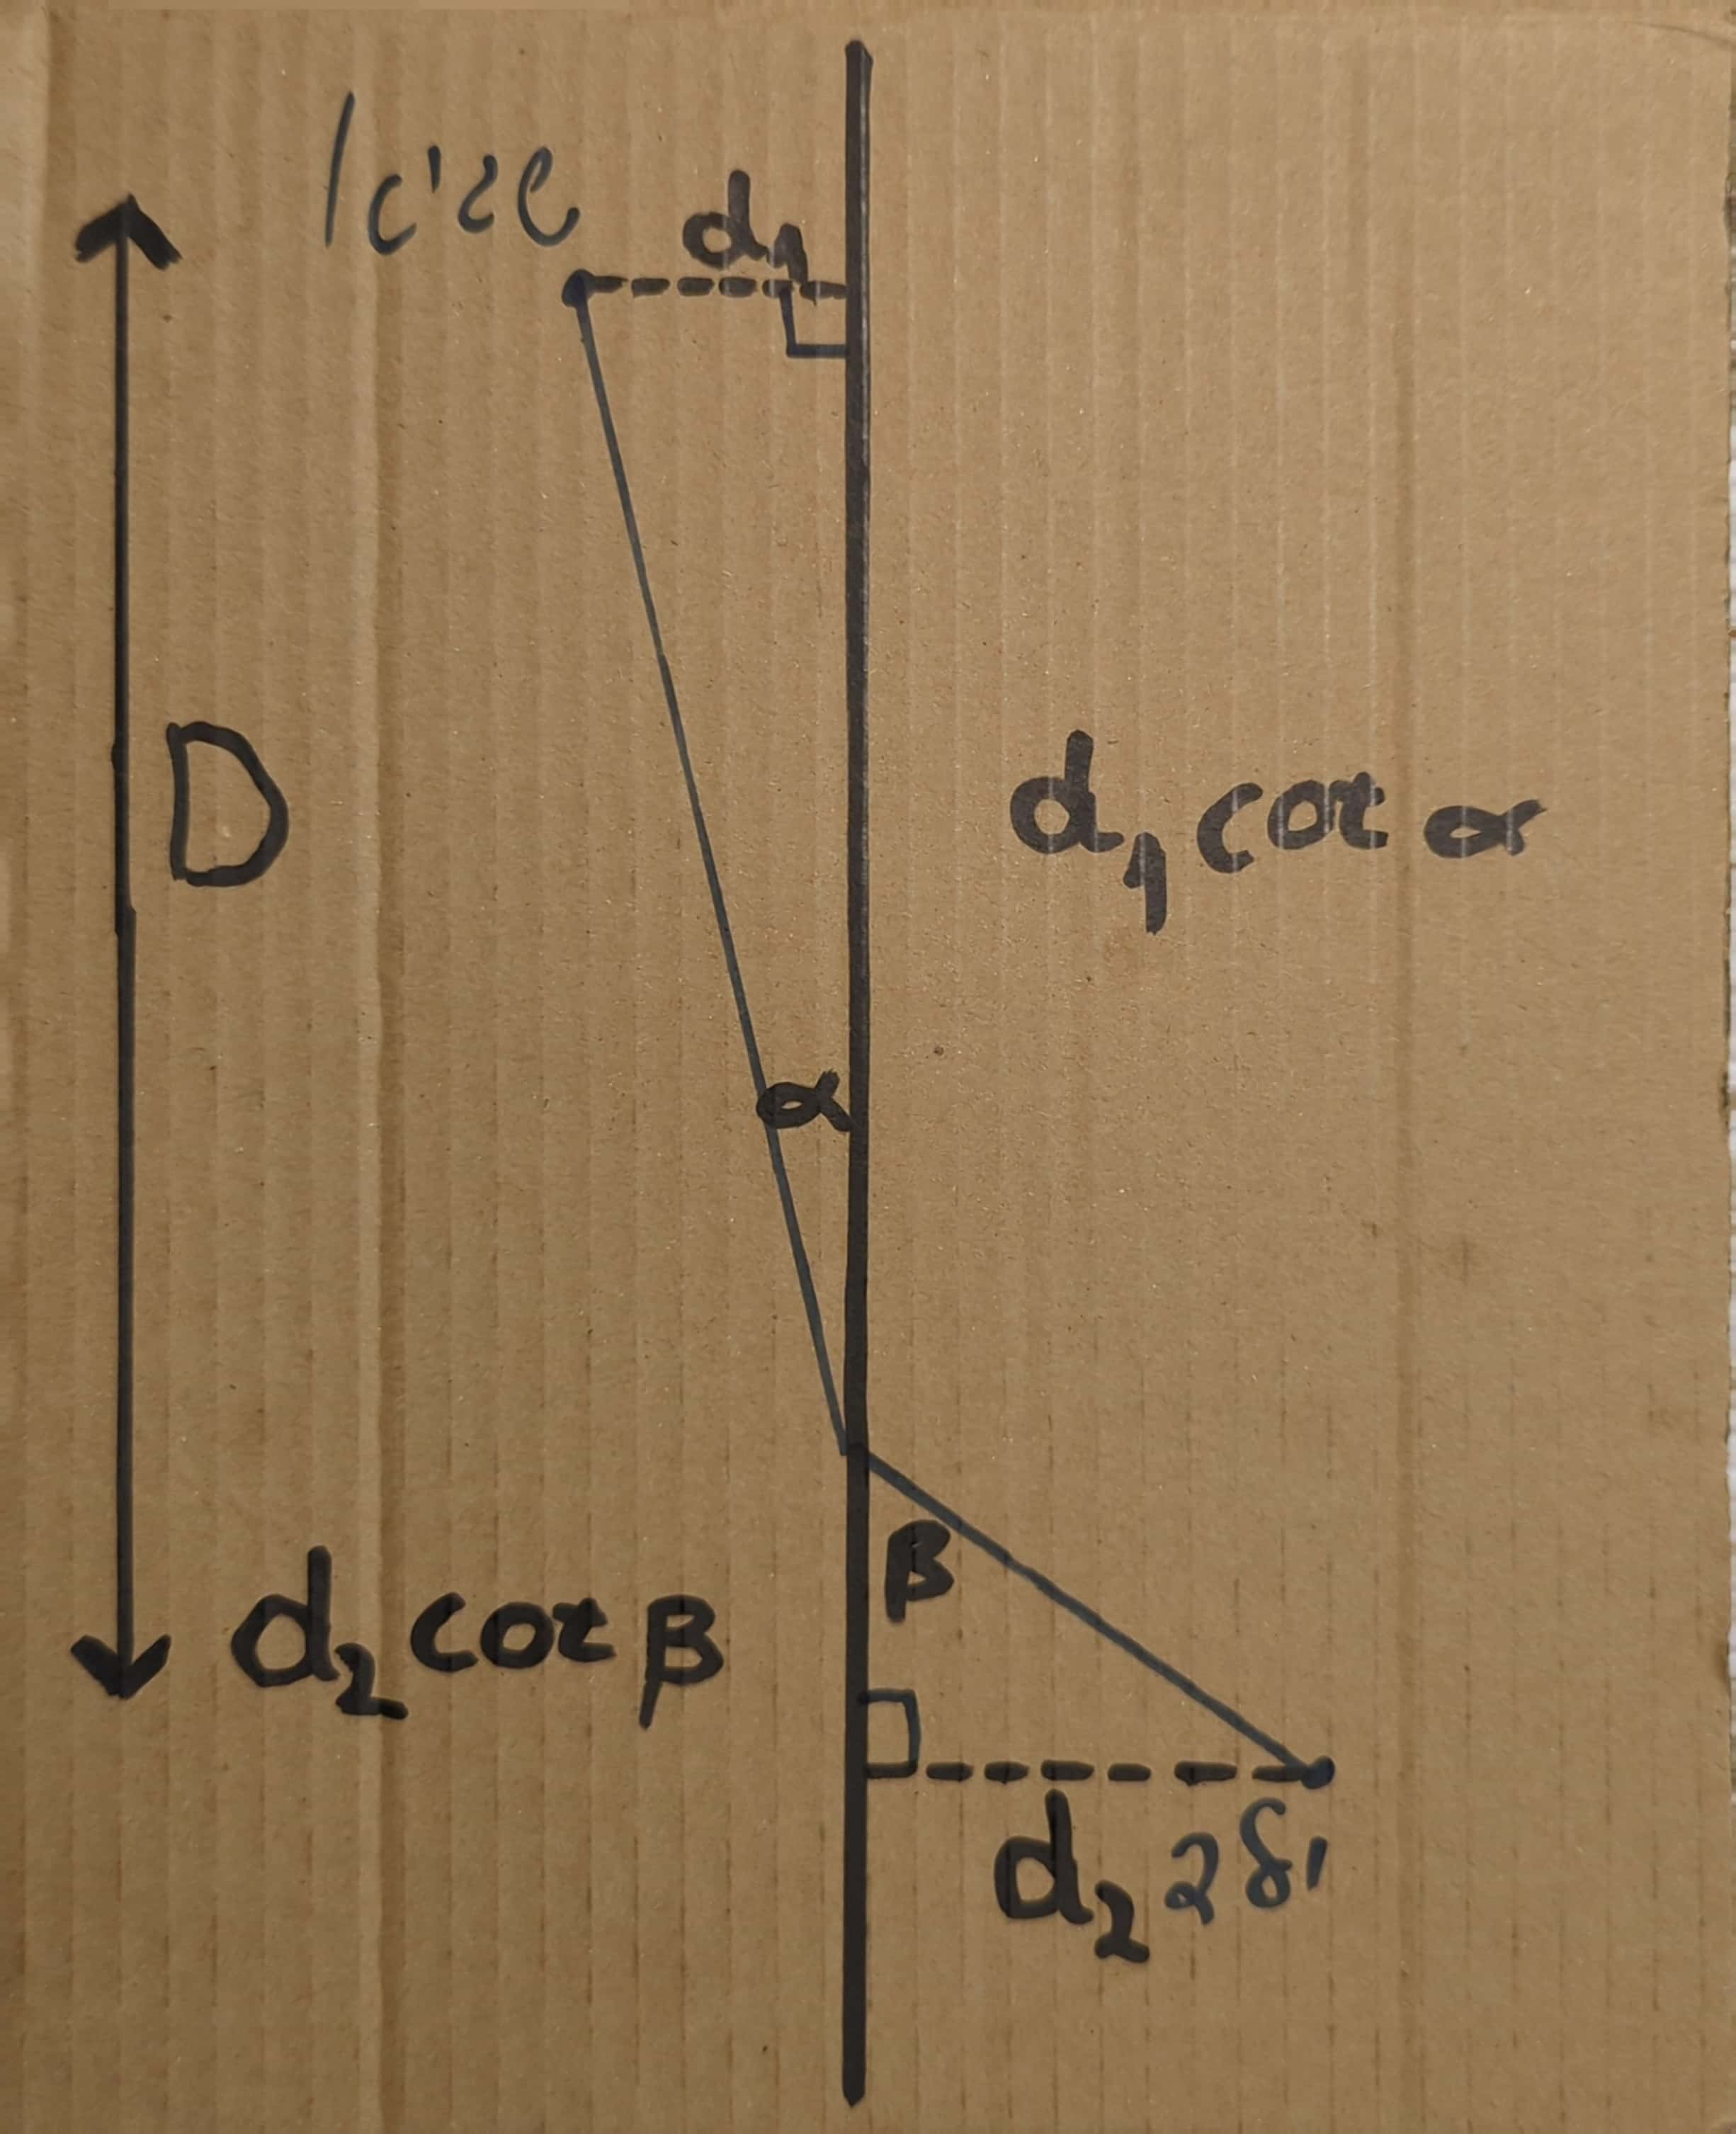
\includegraphics[scale=0.1]{images/CamScanner 10-05-2023 20.48.jpg}
    }
\end{align*}
כלומר:
\begin{flalign*}
    &d_1 \cot \alpha + d_2 \cot \beta = D&&
\end{flalign*}

כלומר התנאים על הזוויות הם:
\begin{empheq}[left=\empheqlbrace]{equation*}
    \begin{flalign*}
        &u\cos{\beta} = v\cos{\alpha}&&\\
        &d_1 \cot \alpha + d_2 \cot \beta = D&&
    \end{flalign*}
\end{empheq}




\end{document}